\documentclass[border=15pt, multi, tikz]{standalone}
\usepackage{import}
\subimport{./layers/}{init}
\usetikzlibrary{positioning}
\usetikzlibrary{3d} %for including external image 

\def\ConvColor{rgb:yellow,5;red,2.5;white,5}
\def\ReLUColor{rgb:yellow,5;red,5;white,5}
\def\BatchNormColor{rgb:red,1;black,0.3}
\def\SEColor{rgb:blue,5;green,2.5;white,5}
\def\DenseColor{rgb:magenta,5;black,7}
\def\LinearColor{rgb:magenta,8;black,7}
\def\AddColor{rgb:blue,5;green,15}

\begin{document}
\setlength{\parindent}{0pt}
\begin{tikzpicture}
\tikzstyle{connection}=[ultra thick,every node/.style={sloped,allow upside down},draw=\edgecolor,opacity=0.7]
\tikzstyle{add_connection}=[ultra thick,every node/.style={sloped,allow upside down},draw=\addcolor,opacity=0.7]
%%%%%%%%%%%%%%%%%%%%%%%%%%%%%%%%%%%%%%%%%%%%%%%%%%%%%%%%%%%%%%%%%%%%%%%%%%%%%%%%%%%%%%%%
%% Draw Layer Blocks
%%%%%%%%%%%%%%%%%%%%%%%%%%%%%%%%%%%%%%%%%%%%%%%%%%%%%%%%%%%%%%%%%%%%%%%%%%%%%%%%%%%%%%%%
\node[canvas is zy plane at x=0] (temp) at (-3,0,0) {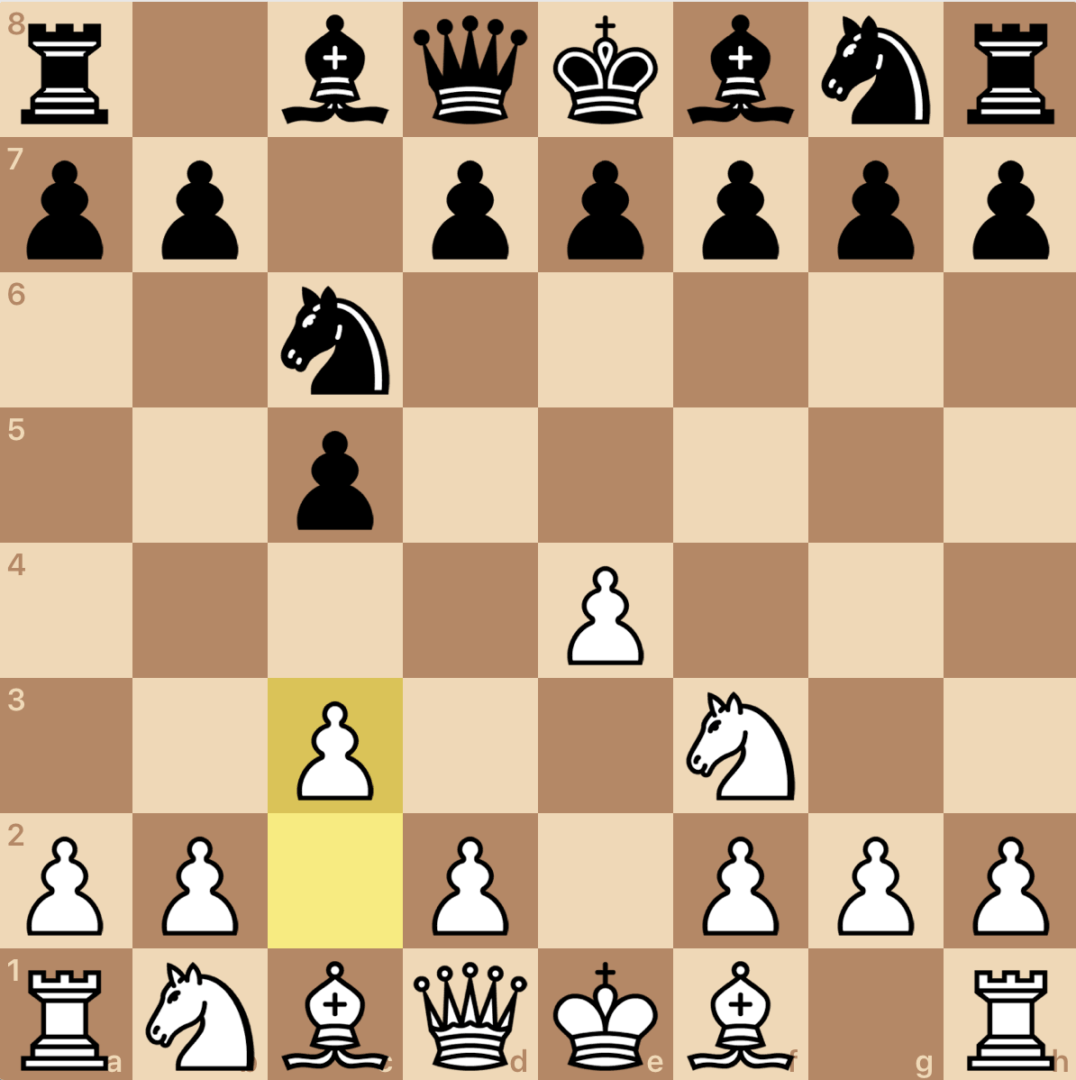
\includegraphics[width=8cm,height=8cm]{chess.png}};

\pic[shift={(0,0,0)}] at (0,0,0) {Box={name=cr1,caption=Conv2D BN ReLU,%
        xlabel={{"64", "dummy"}},fill=\ConvColor,%
        height=40,width=2,depth=40}};
\pic[shift={(0,0,0)}] at (cr1-east) {Box={name=bn1,%
        fill=\BatchNormColor,height=40,width=1,depth=40}};
\pic[shift={(0,0,0)}] at (bn1-east) {Box={name=r1,%
        fill=\ReLUColor,zlabel=8,height=40,width=0.5,depth=40}};

%block 1
\pic[shift={(3,0,0)}] at (r1-east) {Box={name=cr2,caption=Conv2D BN ReLU,%
        xlabel={{"64", "dummy"}},fill=\ConvColor,%
        height=40,width=2,depth=40}};
\pic[shift={(0,0,0)}] at (cr2-east) {Box={name=bn2,%
        fill=\BatchNormColor,height=40,width=1,depth=40}};
\pic[shift={(0,0,0)}] at (bn2-east) {Box={name=r2,%
        fill=\ReLUColor,height=40,width=0.5,depth=40}};

\pic[shift={(1,0,0)}] at (r2-east) {Box={name=cr3,caption=Conv2D\\BN,%
        xlabel={{"64", "dummy"}},fill=\ConvColor,%
        height=40,width=2,depth=40}};
\pic[shift={(0,0,0)}] at (cr3-east) {Box={name=bn3,%
        fill=\BatchNormColor,height=40,width=1,depth=40}};

\pic[shift={(0,5,0)}] at (cr3-east) {Box={name=t1,%
        fill=\ConvColor,height=0,width=0,depth=0}};

\pic[shift={(1,0,0)}] at (bn3-east) {Box={name=se1,caption=SE,%
        xlabel={{"64", "dummy"}},fill=\SEColor,%
        height=40,width=2,depth=40}};

\pic[shift={(1,0,0)}] at (se1-east) {Box={name=addl1,caption=Add\\ReLU,%
        xlabel={{"64", "dummy"}},fill=\AddColor,%
        height=40,width=2,depth=40}};
\pic[shift={(0,-4,0)}] at (addl1-north) {Ball={name=add1,%
        fill=\AddColor,opacity=0.6,%
        radius=2.5,logo=$+$}};
\pic[shift={(0,0,0)}] at (addl1-east) {Box={name=r3,%
        fill=\ReLUColor,zlabel=8,height=40,width=0.5,depth=40}};

%block2
\pic[shift={(3,0,0)}] at (r3-east) {Box={name=cr4,caption=Conv2D BN ReLU,%
        xlabel={{"64", "dummy"}},fill=\ConvColor,%
        height=40,width=2,depth=40}};
\pic[shift={(0,0,0)}] at (cr4-east) {Box={name=bn4,%
        fill=\BatchNormColor,height=40,width=1,depth=40}};
\pic[shift={(0,0,0)}] at (bn4-east) {Box={name=r4,%
        fill=\ReLUColor,height=40,width=0.5,depth=40}};

\pic[shift={(1,0,0)}] at (r4-east) {Box={name=cr5,caption=Conv2D\\BN,%
        xlabel={{"64", "dummy"}},fill=\ConvColor,%
        height=40,width=2,depth=40}};
\pic[shift={(0,0,0)}] at (cr5-east) {Box={name=bn5,%
        fill=\BatchNormColor,height=40,width=1,depth=40}};

\pic[shift={(0,5,0)}] at (cr5-east) {Box={name=t2,%
        fill=\ConvColor,height=0,width=0,depth=0}};

\pic[shift={(1,0,0)}] at (bn5-east) {Box={name=se2,caption=SE,%
        xlabel={{"64", "dummy"}},fill=\SEColor,%
        height=40,width=2,depth=40}};

\pic[shift={(1,0,0)}] at (se2-east) {Box={name=addl2,caption=Add\\ReLU,%
        xlabel={{"64", "dummy"}},fill=\AddColor,%
        height=40,width=2,depth=40}};
\pic[shift={(0,-4,0)}] at (addl2-north) {Ball={name=add2,%
        fill=\AddColor,opacity=0.6,%
        radius=2.5,logo=$+$}};
\pic[shift={(0,0,0)}] at (addl2-east) {Box={name=r5,%
        fill=\ReLUColor,zlabel=8,height=40,width=0.5,depth=40}};

%block3
\pic[shift={(3,0,0)}] at (r5-east) {Box={name=cr6,caption=Conv2D BN ReLU,%
        xlabel={{"64", "dummy"}},fill=\ConvColor,%
        height=40,width=2,depth=40}};
\pic[shift={(0,0,0)}] at (cr6-east) {Box={name=bn6,%
        fill=\BatchNormColor,height=40,width=1,depth=40}};
\pic[shift={(0,0,0)}] at (bn6-east) {Box={name=r6,%
        fill=\ReLUColor,height=40,width=0.5,depth=40}};

\pic[shift={(1,0,0)}] at (r6-east) {Box={name=cr7,caption=Conv2D\\BN,%
        xlabel={{"64", "dummy"}},fill=\ConvColor,%
        height=40,width=2,depth=40}};
\pic[shift={(0,0,0)}] at (cr7-east) {Box={name=bn7,%
        fill=\BatchNormColor,height=40,width=1,depth=40}};

\pic[shift={(0,5,0)}] at (cr7-east) {Box={name=t3,%
        fill=\ConvColor,height=0,width=0,depth=0}};

\pic[shift={(1,0,0)}] at (bn7-east) {Box={name=se3,caption=SE,%
        xlabel={{"64", "dummy"}},fill=\SEColor,%
        height=40,width=2,depth=40}};

\pic[shift={(1,0,0)}] at (se3-east) {Box={name=addl3,caption=Add\\ReLU,%
        xlabel={{"64", "dummy"}},fill=\AddColor,%
        height=40,width=2,depth=40}};
\pic[shift={(0,-4,0)}] at (addl3-north) {Ball={name=add3,%
        fill=\AddColor,opacity=0.6,%
        radius=2.5,logo=$+$}};
\pic[shift={(0,0,0)}] at (addl3-east) {Box={name=r7,%
        fill=\ReLUColor,zlabel=8,height=40,width=0.5,depth=40}};

%block4
\pic[shift={(3,0,0)}] at (r7-east) {Box={name=cr8,caption=Conv2D BN ReLU,%
        xlabel={{"64", "dummy"}},fill=\ConvColor,%
        height=40,width=2,depth=40}};
\pic[shift={(0,0,0)}] at (cr8-east) {Box={name=bn8,%
        fill=\BatchNormColor,height=40,width=1,depth=40}};
\pic[shift={(0,0,0)}] at (bn8-east) {Box={name=r8,%
        fill=\ReLUColor,height=40,width=0.5,depth=40}};

\pic[shift={(1,0,0)}] at (r8-east) {Box={name=cr9,caption=Conv2D\\BN,%
        xlabel={{"64", "dummy"}},fill=\ConvColor,%
        height=40,width=2,depth=40}};
\pic[shift={(0,0,0)}] at (cr9-east) {Box={name=bn9,%
        fill=\BatchNormColor,height=40,width=1,depth=40}};

\pic[shift={(0,5,0)}] at (cr9-east) {Box={name=t4,%
        fill=\ConvColor,height=0,width=0,depth=0}};

\pic[shift={(1,0,0)}] at (bn9-east) {Box={name=se4,caption=SE,%
        xlabel={{"64", "dummy"}},fill=\SEColor,%
        height=40,width=2,depth=40}};

\pic[shift={(1,0,0)}] at (se4-east) {Box={name=addl4,caption=Add\\ReLU,%
        xlabel={{"64", "dummy"}},fill=\AddColor,%
        height=40,width=2,depth=40}};
\pic[shift={(0,-4,0)}] at (addl4-north) {Ball={name=add4,%
        fill=\AddColor,opacity=0.6,%
        radius=2.5,logo=$+$}};
\pic[shift={(0,0,0)}] at (addl4-east) {Box={name=r9,%
        fill=\ReLUColor,zlabel=8,height=40,width=0.5,depth=40}};
        

\pic[shift={(3,0,0)}] at (add4-east) {Box={name=cr10,caption=Conv2D BN ReLU,%
        xlabel={{"64", "dummy"}},fill=\ConvColor,%
        height=40,width=2,depth=40}};
\pic[shift={(0,0,0)}] at (cr10-east) {Box={name=bn10,%
        fill=\BatchNormColor,height=40,width=1,depth=40}};
\pic[shift={(0,0,0)}] at (bn10-east) {Box={name=r10,%
        fill=\ReLUColor,zlabel=8,height=40,width=0.5,depth=40}};

\pic[shift={(3,0,0)}] at (r10-east) {Box={name=f1,caption=Flatten,%
        xlabel={{"4096", "dummy"}},fill=\DenseColor,%
        zlabel=1,height=5,width=20,depth=5}};

\pic[shift={(3,0,0)}] at (f1-east) {RightBandedBox={name=fl1,caption=Fully connected Linear,%
        xlabel={{"1", "dummy"}},fill=\DenseColor,bandfill=\LinearColor,%
        zlabel=1,height=5,width=5,depth=5}};

\pic[shift={(3,0,0)}] at (fl1-east) {Box={name=v1,caption=Evaluation,%
        xlabel={{"1", "dummy"}},fill=\DenseColor,%
        zlabel=1,height=5,width=5,depth=5}};

%%%%%%%%%%%%%%%%%%%%%%%%%%%%%%%%%%%%%%%%%%%%%%%%%%%%%%%%%%%%%%%%%%%%%%%%%%%%%%%%%%%%%%%%
%% Draw connections
%%%%%%%%%%%%%%%%%%%%%%%%%%%%%%%%%%%%%%%%%%%%%%%%%%%%%%%%%%%%%%%%%%%%%%%%%%%%%%%%%%%%%%%%
\draw [connection]  (r1-east)    -- node {\midarrow} (cr2-west);

\draw [connection]  (r2-east)    -- node {\midarrow} (cr3-west);
\draw [connection]  (bn3-east)    -- node {\midarrow} (se1-west);
\draw [connection]  (se1-east)    -- node {\midarrow} (add1-west);

\draw [connection]  (r3-east) -- node {\midarrow} (cr4-west);

\draw [connection]  (r4-east)    -- node {\midarrow} (cr5-west);
\draw [connection]  (bn5-east)    -- node {\midarrow} (se2-west);
\draw [connection]  (se2-east)    -- node {\midarrow} (add2-west);

\draw [connection]  (r5-east) -- node {\midarrow} (cr6-west);

\draw [connection]  (r6-east)    -- node {\midarrow} (cr7-west);
\draw [connection]  (bn7-east)    -- node {\midarrow} (se3-west);
\draw [connection]  (se3-east)    -- node {\midarrow} (add3-west);

\draw [connection]  (r7-east) -- node {\midarrow} (cr8-west);

\draw [connection]  (r8-east)    -- node {\midarrow} (cr9-west);
\draw [connection]  (bn9-east)    -- node {\midarrow} (se4-west);
\draw [connection]  (se4-east)    -- node {\midarrow} (add4-west);

\draw [connection]  (add4-east)    -- node {\midarrow} (cr10-west);
\draw [connection]  (r10-east)    -- node {\midarrow} (f1-west);
\draw [connection]  (f1-east)    -- node {\midarrow} (fl1-west);
\draw [connection]  (fl1-east)    -- node {\midarrow} (v1-west);


\path (cr2-north) -- (addl1-north) coordinate[pos=0] (between1_2) ;
\draw [add_connection]  (between1_2)    -- node {\addarrow} (t1-west-|between1_2) -- node {\addarrow} (t1-west);
\draw [add_connection]  (t1-east) -- node {\addarrow} (t1-east-|addl1-north)-- node {\addarrow} (addl1-north);

\path (cr4-north) -- (addl2-north) coordinate[pos=0] (between3_4) ;
\draw [add_connection]  (between3_4)    -- node {\addarrow} (t2-west-|between3_4) -- node {\addarrow} (t2-west);
\draw [add_connection]  (t2-east) -- node {\addarrow} (t2-east-|addl2-north)-- node {\addarrow} (addl2-north);

\path (cr6-north) -- (addl3-north) coordinate[pos=0] (between5_6) ;
\draw [add_connection]  (between5_6)    -- node {\addarrow} (t3-west-|between5_6) -- node {\addarrow} (t3-west);
\draw [add_connection]  (t3-east) -- node {\addarrow} (t3-east-|addl3-north)-- node {\addarrow} (addl3-north);

\path (cr8-north) -- (addl4-north) coordinate[pos=0] (between7_8) ;
\draw [add_connection]  (between7_8)    -- node {\addarrow} (t4-west-|between7_8) -- node {\addarrow} (t4-west);
\draw [add_connection]  (t4-east) -- node {\addarrow} (t4-east-|addl4-north)-- node {\addarrow} (addl4-north);

\draw[densely dashed]
(r10-nearnortheast) -- (f1-nearnorthwest)
(r10-nearsoutheast) -- (f1-nearsouthwest)
(r10-farsoutheast)  -- (f1-farsouthwest)
(r10-farnortheast)  -- (f1-farnorthwest)
;

\end{tikzpicture}
\end{document}\grid
